%% Be sure to check spelling!

%% Put your name and the proper due date in place

%% Copy the lstinputlisting and figure code as many times as you need
%% Be sure to put in your own file names if appropriate

%% Note that the \includegraphics and \lstinputlisting commands
%% are currently commented out with %%% - until the
%% files exist, processing this code without them will result in an error
%% so leave the comments until you have created the files!

\documentclass{article}
\usepackage{amsmath}    % loads AMS-Math package
\usepackage{graphicx}   % bring in graphics
\usepackage{listings}   % allows lstlisting environment
\usepackage[letterpaper, margin=0.5in]{geometry}  % set paper size/margins
\usepackage{EGR103style}  % colorful file imports

\begin{document}
\begin{center}
\rule{6.5in}{0.5mm}\\~\\
\textbf{\large EGR 103L -- Fall 2021}\\~\\
\textbf{\huge Laboratory 9 - Curve Fitting}\\~\\
**NAME (NET ID)**\\
Lab Section **NUMBER AND LETTER**, **DAY AND TIMES**\\
**DATEDUE**, **YEAR**\\~\\
{\small I have adhered to the Duke Community Standard in completing this assignment.  I understand that a violation of the Standard can result in failure of this assignment, failure of this course, and/or suspension from Duke University.} 
\rule{6.5in}{0.5mm}\\
\end{center}
\tableofcontents
\listoffigures
\renewcommand{\arraystretch}{1.5}
\clearpage

\section{Chapra 14.5}
\begin{center}
\begin{tabular}{l|c|c|c|c|c|c}
Case & Equation & $S_t$ & $S_r$ & $r^2$ & $s$ & $r$ \\ \hline
$y$ vs. $x$ & $y=~x+~$ & ~ & 
~ & ~ & ~ & ~\\ 
$x$ vs. $y$ & $x=~y+~$ & ~ & 
~ & ~ & ~ & ~
\end{tabular}
\end{center}
%%% Replace the ~ above with your values 
%%% Discussion

\section{Chapra 14.7}
\begin{center}
\begin{tabular}{c|c|c|c}
$S_t$ & $S_r$ & $r^2$ & $R$, N m mol$^{-1}$ K$^{-1}$ or J  mol$^{-1}$ K$^{-1}$\\ \hline
~ & ~  & ~ & ~
\end{tabular}
\end{center}
%%% Replace the ~ above with your values 
%%% Discussion / reference for R value

\section{Chapra 14.27}
\begin{center}
\begin{tabular}{l|c|c|c|c|c}
Case & Equation & $S_t$ & $S_r$ & $r^2$ & $i(3.5)$, A\\ \hline
Polyfit & $i=~v+~$ & ~ & 
~ & ~ & ~\\ 
Genlin & $i=~v$ & ~ &
~ & ~ & ~
\end{tabular}
\end{center}
%%% Replace the ~ above with your values 
%%% Discussion 

\section{Chapra 15.10}
Based on the least squares fit of the given model,
\begin{align*}
p(t)&=~e^{-1.5t} + ~e^{-0.3t} + ~e^{-0.05t}
\end{align*}
% Disccusion
The statistical and information required by the problem is:
\begin{center}
\begin{tabular}{c|c|c}
$S_t$ & $S_r$ & $r^2$\\ \hline
~ & ~ & ~ \\
\end{tabular}
\end{center}
%%% Replace the ~ above with your values 
%%% Discussion 

\section{Chapra 15.10 Alternate}
Based on the least squares fit of the given model,
\begin{align*}
p(t)&=~e^{-1.5t} + ~e^{-0.3t} + ~e^{-0.2t}
\end{align*}
% Disccusion
The statistical and specific information required by the problem is:
\begin{center}
\begin{tabular}{c|c|c}
$S_t$ & $S_r$ & $r^2$\\ \hline
~ & ~ & ~ \\
\end{tabular}
\end{center}
%%% Replace the ~ above with your values 
%%% Discussion 

\section{Chapra 15.5}
With the chloride concentration equal to 0, a cubic fit of the oxygen concentration yields:
\begin{align*}
\hat{OC}(0, T)&=
(~)\,T^3  
(~)\,T^2 
(~)\,T  
(~)
\end{align*}
\begin{center}
\begin{tabular}{c|c|c}
$S_t$ & $S_r$ & $r^2$  \\ \hline
~& ~ & ~
\end{tabular}
\end{center}
%%% Replace the ~ above with your values 
%%% Put the appropriate sign in front of each coefficient
%%% Discussion 

\section{Chapra 15.6}
Using a planar model:
\begin{align*}
\hat{OC}(c, T)&=\sum_ma_m\phi_m(c, T)=a_0(c^0T^0)+a_1(c^1)+a_2(T^1)
\end{align*}
the model coefficients and other required values are:
\begin{center}
\begin{tabular}{c|c|c|c|c|c}
$a_0$ & $a_1$ & $a_2$ & $r^2$ & $OC(15, 12)$ g/ml & $\epsilon_t$ \\ \hline
~ & ~ & ~ & ~ & ~ & ~\%
\end{tabular}
\end{center}

%%% Replace the ~ above with your values 
%%% Discussion 

\section{Chapra 15.7}
Using a first-order model for $c$ and a third-order model for $T$:
\begin{align*}
\hat{OC}(c, T)&=
\sum_ma_m\phi_m(c, T)=a_0(c^0T^0)+a_1(c^1)+a_2(T^3)+a_3(T^2)+a_4(T^1) 
\end{align*}
the model coefficients and other required values are:
\begin{center}
\begin{tabular}{c|c|c|c|c|c|c|c}
$a_0$ & $a_1$ & $a_2$ & $a_3$ & $a_4$ & $r^2$ & $OC(15, 12)$ g/ml & $\epsilon_t$ \\ \hline
~ & ~ & ~ & ~ & ~ & ~ & ~ & ~\%
\end{tabular}
\end{center}

%%% Replace the ~ above with your values 
%%% Discussion 

\pagebreak
\appendix
\section{Codes}
% Put the name of your file in the subsection name 
% and the listinginput input
% Be sure to include the community standard in codes!
% Add \pagebreaks if they make sense
% Make as many copies as you need
\lstset{style=python103, language=python} 

\subsection{Chapra 14.5}
%%%\lstinputlisting{chapra_14_005.py}
\pagebreak

\subsection{Chapra 14.7}
%%%\lstinputlisting{chapra_14_007.py}
\pagebreak

\subsection{Chapra 14.27}
%%%\lstinputlisting{chapra_14_027.py}
\pagebreak

\subsection{Chapra 15.10}
%%%\lstinputlisting{chapra_15_010.py}
\pagebreak

\subsection{Chapra 15.10 Alternate}
%%%\lstinputlisting{chapra_15_010alt.py}
\pagebreak

\subsection{Chapra 15.005}
%%%\lstinputlisting{chapra_15_005.py}
\pagebreak

\subsection{Chapra 15.006}
%%%\lstinputlisting{chapra_15_006.py}
\pagebreak

\subsection{Chapra 15.007}
%%%\lstinputlisting{chapra_15_007.py}
\pagebreak

\section{Figures}
% Make as many as needed; change sizes if it makes sense to do so
\begin{figure}[h!]
\begin{center}
%%%\includegraphics{chapra_14_005_plot.png}
\caption{Chapra 14.5}
\end{center}
\end{figure}
 
\begin{figure}[htb!]
\begin{center}
%%%\includegraphics{chapra_14_027_plot.png}
\caption{Chapra 14.27}
\end{center}
\end{figure}


\begin{figure}[htb!]
\begin{center}
%%%\includegraphics{chapra_15_010_plot.png} \\
%%%\includegraphics{chapra_15_010alt_plot.png}
\caption{Chapra 15.10 and 15.10 Alternate}
\end{center}
\end{figure}

\begin{figure}[htb!]
\begin{center}
%%%\includegraphics{chapra_15_005_plot.png}
\caption{Chapra 15.5}
\end{center}
\end{figure}

\begin{figure}[htb!]
\begin{center}
%%%\includegraphics{chapra_15_006_plot1.png}\\
%%%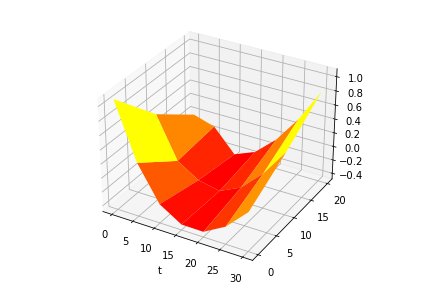
\includegraphics{chapra_15_006_plot2.png}
\caption{Chapra 15.6}
\end{center}
\end{figure}

\begin{figure}[htb!]
\begin{center}
%%%\includegraphics{chapra_15_007_plot1.png}\\
%%%\includegraphics{chapra_15_007_plot2.png}
\caption{Chapra 15.7}
\end{center}
\end{figure}

\end{document}
